\documentclass[11pt]{article}
\usepackage[margin = 1in, paperwidth = 8.5in, paperheight = 11in]{geometry}
\usepackage{amsfonts}
\usepackage{amsmath}
\usepackage{indentfirst}
\usepackage{graphicx}
\usepackage{color}
\usepackage[procnames]{listings}

\graphicspath{{/Users/whatever/Documents/Practicals/CS181/}}
\title{CS181 Practical 1 \\ Predicting the Efficiency of Organic Photovoltaics}
\author{Zhou Yu, Brendan Bozorgmir, Kevin Rankine - Kaggle Team: MachineLearnersYeah}

\begin{document}
\maketitle
\newpage
\tableofcontents
\newpage
\section{Select Meaningful Features}
We begin by roughly examining the training data set. Our goal is to select a subset of the features that can represent the whole feature set and has a tolerable dimensionality. Apparently the training data set has too many dimensions and too many sample points to be visualized directly. Instead we use some very simple statistics to assess the likelyhood of a particular feature to be informative. One way is to look how wide/narrow the distribution of a given feature is. The most naive way to do this is to obtain the maximum and minimum values of a feature. A plot of the maximum and minimum values of all 256 features are plotted below. Maxima are denoted by red dots and minima green dots.
\begin{figure}[h!]
\centering
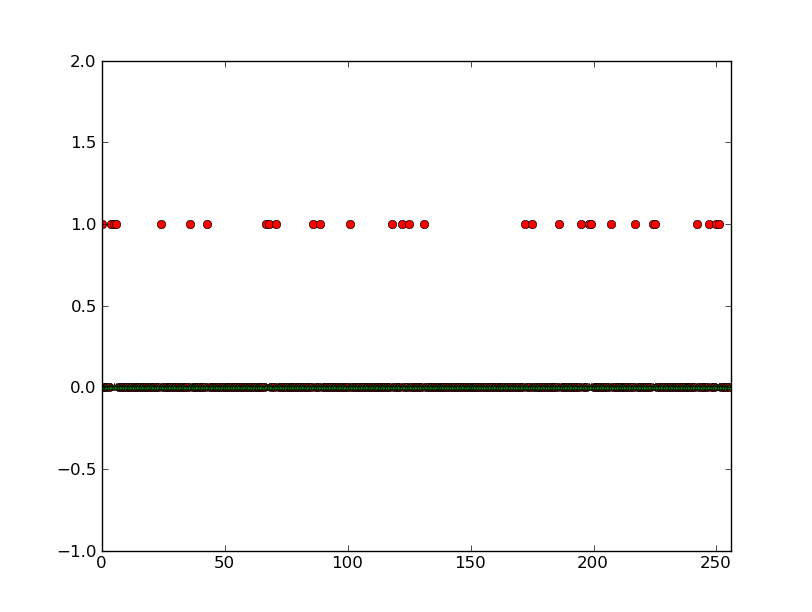
\includegraphics[scale=0.5]{examining_min_and_max.png}
\caption{Min and Max of All 256 Features}
\end{figure}
Surprisingly we have found that only a small subset of all features are actually multivalued. Most of the values adopt 0 over all sample points. Obviously taking these features into account cannot improve the learning process as they provide no information, so we only need to take non-zero features into account. Collecting all non-zero features we found that only the follow 31 features have a binary value of zero or one:

\begin{center}
[ 0, 4, 5, 6, 24, 36, 43, 67, 67, 68, 71, 86, 89, 101, \\
118, 122, 125, 131, 172, 175, 186, 195, 198, 199, \\ 207, 217, 224,
225, 242, 247, 250, 251 ]
\end{center}

We then conducted a F-test to determine whether choosing 0 or 1 for a particular feature significantly affect the gap energy of a molecule. Among the 31 features we found that only feature number 4 fails to cause a significant change in molecular gap energy ($p >= 0.05$). Thus this feature is also discarded.Given that 31 is a sufficiently small number, at the current stage we will not perform any further selection on the parameters.
\\

However, we went further than this with our feature engineering, because we noted that regardless of the actual tools (variants of regression with basis functions or a support vector machine) we used to model the data, we were still getting testing data set errors that were within the range $.25 - .29$. We noted that the original features were generated from the SMILE strings based on the following command:

\definecolor{keywords}{RGB}{255,0,90}
\definecolor{comments}{RGB}{0,0,113}
\definecolor{red}{RGB}{160,0,0}
\definecolor{green}{RGB}{0,150,0}
 
\lstset{language=Python, 
        basicstyle=\ttfamily\small, 
        keywordstyle=\color{keywords},
        commentstyle=\color{comments},
        stringstyle=\color{red},
        showstringspaces=false,
        identifierstyle=\color{green},
        procnamekeys={def,class}}
 
\begin{lstlisting}
  AllChem.GetMorganFingerprintAsBitVect( MolFromSmiles( molecule ), 1, nBits= 256,
       useFeatures = True)
\end{lstlisting}
We altered this to the following command:

\lstset{language=Python,
        basicstyle=\ttfamily\small,
        keywordstyle=\color{keywords},
        commentstyle=\color{comments},
        stringstyle=\color{red},
        showstringspaces=false,
        identifierstyle=\color{green},
        procnamekeys={def,class}}

\begin{lstlisting}
  AllChem.GetMorganFingerprintAsBitVect( MolFromSmiles( mol ), 2, nBits= 512)
\end{lstlisting}

This essentially gave us more features to work with, and we found it ultimately made our predictions significantly more accurate. We then performed all the feature selection (F-test and variance analysis of individual features) above on this new feature set in the same manner as we performed it on the old feature set. We ended up using 10000 training samples for all our methods, each with 275 features left over after our feature engineering. Using the radial basis functions discussed in the next section, we were able to increase the number of features to 775 for each sample (including the original 275 features) when using all our methods except for SVM. We used scikit-learn modules for all of our algorithms.


\section{Linear Regression}
Linear regression is the simplest possible way to fit the training data and obtain a model to predict the test data. In order to use linear regression to represent non-linear features in the data basis functions must be carefully chosen. To avoid overfitting, regularization terms should be introduced to limit the magnitude of regression coefficients. The exact value of the penalty strength parameter can be chosen by cross validation. Finally, to account for uncertainty in the model, we can adopt a Bayesian probabilistic view and average out the uncertainty in regression coefficients. In this section we will address these issues one by one.
\subsection{Choose Basis Functions}\label{choose basis function}
Common basis function forms include polynomial basis, sigmoidal basis, sinosoidal basis and Gaussian basis. Among all these only gaussian basis functions decay rapidly away from the center and can be easily generalized to high dimensions and thus preferable for our model. A multivariant Gaussian basis function takes the form:
$$f(\textbf{x}) = \exp \left(-\frac{(\textbf{x} - \boldsymbol{\mu})^2}{r^2}\right)$$
where $\boldsymbol{\mu}$ denotes the center of the basis function and $r$ denotes the radius of the function. 

Given this, choosing the basis functions is equivalent to choosing appropriate centers and radius. Intuitively, the center of a basis function represents a center of a cluster of data points that share roughly the same properties, whereas the radius of that basis function represents how wide the data points spread. Based on such an intuition, we can use unsupervised classification of the data points to obtain clusters and calculate the center and radius based on the classification.

Here we use K-Means classification as an unsupervised classification method to find data clusters. This method can be replaced by more robust methods such as support vector classification to give better results. In a K-Means classification, the user specifies a number $N$ as the number of clusters to be classified. Here $N$ corresponds to the number of basis functions we want to have. Then $N$ random centers are generated and data are clustered based on proximity to those centers. Then new centers are generated as the mean of the data in that class and data are re-clustered based on new centers. This will iterate until centers no longer shift significantly. After convergence, the centers of the $N$ clusters will serve as $\boldsymbol{\mu}$ in basis functions. To determine radius of basis functions, square distances between centers are calculated.
$$d_{ij} = ||\boldsymbol{\mu_i} - \boldsymbol{\mu_j}||^2, i \neq j, \ i,j \in \{1, 2, ..., N \}$$
Based on these sqaure distances we find for each $\boldsymbol{\mu_i}$ its $K$ nearest neighbours and calculate the mean distance between $\boldsymbol{\mu_i}$ and its nearest neighbours. This distance will serve as the radius.
$$r_i = \sqrt{\frac{\sum_{k = 1}^K d_{i,nearest_k}}{K}}$$
Using this method, once we specify cluster number $N$ and neighbour number $K$, we can get $N$ Gaussian basis functions that match the geometry of the data. As to the number of basis functions, tradeoff must be made between model accuracy and computation complexity. In this work, the number of basis functions for linear regression will be set at 500.

\subsection{Regularized Linear Regression}\label{linear regression}
Regularized linear regression, including Ridge regression, Lasso regression and their combination elastic network restrict model complexity by introducing a regularization term that penalize coefficient vectors with large norms: 
\begin{eqnarray}
E(\textbf{w}) &=& E_D(\textbf{w}) + E_\textbf{w}(w) \\
              &=& \frac{1}{2}\sum_{n=1}^N(t_n - \textbf{w}^T\boldsymbol{\phi} (\textbf{x}_n)) + \lambda||\textbf{w}||_p^p
\end{eqnarray}
where $||w||_p^p$ donotes the $L_p$ norm used in the corresponding method. The difference between these three models is the way norm is claculated. Ridge regression uses $L_2$ norm while Lasso regression uses $L_1$ norm and elastic network incorporates both of them. Here we will use all three of them and compare their performances.

For all three regression methods, basis functions are chosen as discussed in section \ref{choose basis function} The number of Gaussian basis function is always 500. In addition to Gaussian basis, linear basis is also included. Given there are 275 features, the total number of basis function features is 775. 

To train the model, we sectioned the training data into two parts, the first includes the first 10000 sample points and is used as training data set and the second includes the next 5000 sample points and is used as test data set to evaluate performance. The rest of the data is discarded to save time in training our models. 

For all three methods, K-folds cross validation is used to choose the $\lambda$ in the regularization term in order to give a best balance between model complexity and the accuracy of data fitting. The 10000 training data are radomly divided into 10 parts and for cross validation the model is trained on 9 parts of the data and validated on the 10th part.

For each method, the trained model was used to predict the energy gap for both training data and testing data. The average error is calculated based on
$$E_{avg} = \sqrt{\frac{\sum_{n = 1}^{N}(EG_{real} - EG_{predicted})^2}{N}}$$
for both the training and testing data to assess the accuracy of the model.Results of regularized linear regression are summarized below.

For Ridge regression, $\lambda$ was first chosen among 0.01, 0.1, 1, and 10, with 0.1 giving the best result. Using $\lambda = 0.1$ as the penalty strength, the average error in the training data set is $\approx .149$ while the average error in the testing data set is $\approx 0.159$. The less than small differece between the average error calculated on training and testing data sets indicates that the model faithfully represents the true features in the data sets.

For Lasso regression, $ \lambda $ was chosen among a wide range of values including $ 10^{-7}, 5\times 10^{-7}, 10^{-6}, 5\times 10^{-6}, 10^{-5}, 10^{-4}, 0.001, 0.01, 0.1$ and $1$, with $10^{-5}$ giving the best result. Note that the exceeding small value of $\lambda$ is due to the fact that in Lasso regression the term $E_D(\textbf{w})$ is scaled based on the number of data points. Using $\lambda = 10^{-5}$, the average error calculated in training data set is $\approx 0.151$ while the average error calculated in testing data set is $\approx 0.161$. Again the result is consistent.

For elastic network regression, instead of choosing specific values of penalty against $L_1$ norm and $L_2$ norm, we choose the ratio between these two. Using cross validation to choose among $0, 0.2, 0.5, 0.7, 0.9, 0.95, 0.99$ and $1$, $1$ was finally selected. This means that the elastic network retrogrades into Lasso regression. Thus we shall simply use the result of Lasso regression to represent the result of elastic network regression. 

\subsection{Bayesian Linear Regression}
We have seen in the course that assuming a Gaussian prior for the regression coefficients and a Gaussain noise model the bayesian regression problem is related to a Ridge regression problem. However, if we again introduce prior for the hyperparameters in the prior as well as the noise model, marginal likelyhood can be calculated and we can estimate the best hyperparameters by maximizing marginal likelyhood. Potentially this can give better result. In a Gaussian prior of regression coefficients we always assume zero mean. For analytic convenience we assume that the precision follows a $\gamma$ distribution, which is the conjugate prior for Gaussian distribution. Similarly we assume a $\gamma$ distribution for the precision of noise model. 

If we assume different regression coefficients are independent and have the same precision, then apart from the hyper prior, the bayesian model is equivalent to a Ridge regression model. To determine the parameters for the hyper priors, namely the shape and scale parameters for the two $\gamma$ distributions, we used cross validation as described in section \ref{linear regression}. We found that over a wide range ($10^{-7} \sim 10^{-5}$) the parameters in hyper priors have little effect on the final result. Thus we chose default value to train the model using the 700000 samples data set. The average error calculated in training data set is $0.149942172314$ and the average error calculated in testing data set is $0.160946582136$. This is quite comparable to the result of Ridge regression.

\section{Support Vector Regression}

SVR operates in a manner similar to other regression models, yet different in that the process of training the (simplest version of) the SVR consists of minimizing the $L_2$ norm of the weights subject to a set of equations (for each $i$): $t_i -  \langle \textbf{w}, \textbf{x}_i\rangle\ \leq \epsilon $, $\langle \textbf{w}, \textbf{x}_i \rangle\ + b - t_i \leq \epsilon$, with $\langle \textbf{w}, \textbf{x}_i\rangle\ + b$ as the predicted value of the SVR model on $\textbf{x}_i$, where we define $\langle \textbf{x}, \textbf{y} \rangle = exp(\gamma||x - y||^2)$ (this is called an RBF kernel). We used the default value of epsilon and C provided by scikit-learn ($0.1$ and $1$), but we performed fivefold cross validation (in the same manner as we did for the other regression models) to determine the optimal parameter of $\gamma$ (a value used in the kernel function for the SVR). We chose among the set $\{0.01, 0.05, 0.1, 0.5, 1\}$ and found that $\gamma = 0.05$ yielded the best results, with an error of $\approx 0.076$ on the training data set and an error of $0.125$ on the testing data set.

\section{Conclusions}

We ultimately ended up using the Support Vector Regression method for the Kaggle competition, which yielded an error of $0.08236$.

The summary of our errors is listed in the table below:

\begin{tabular}{| l ||  c | r |}
	\hline
  \textbf{ } & Error on Training & Error on Testing \\ \hline
  Ridge Regression & .149 & .159 \\\hline
  Lasso Regression & .151 & .161 \\\hline
  Elastic Network Regression & .151 & .161\\ \hline
	Bayesian Linear Regression & .150 & .161 \\\hline
	Support Vector Regression & .076 & 0.125 \\\hline
\end{tabular}

Throughout this practical, we found that the determinative factor of the success of our predictions lay mostly in our feature selection and engineering. Without that, the predictive error for each of the models was not too far of from the predictive error of the other models. In that sense, the critical aspect of this project wasn't really the model we chose, but ultimately how we selected and modified our features based on the original SMILE strings.


\end{document}
